\chapter{The BONuS12 Experiment}
\label{ch:bonus}
The BONuS12 Experiment will be conducted at the Thomas Jefferson National Laboratory (JLab) in Newport News, Virginia. JLab was founded in 1984 with the intent of studying the structure of nuclear matter. The unique accelerator that was built at JLab, called the Continuous Electron Beam Accelerator Facility (CEBAF), allowed for the realization of that intent by providing for the probing of atomic nuclei at the quark level. In order to understand the BONuS12 Experiment, we must first understand CEBAF and the Hall B spectrometer that the BONuS12 RTPC will be installed in. Then we will discuss the RTPC design, components, and construction.

\begin{figure}[h!]
	\centering
	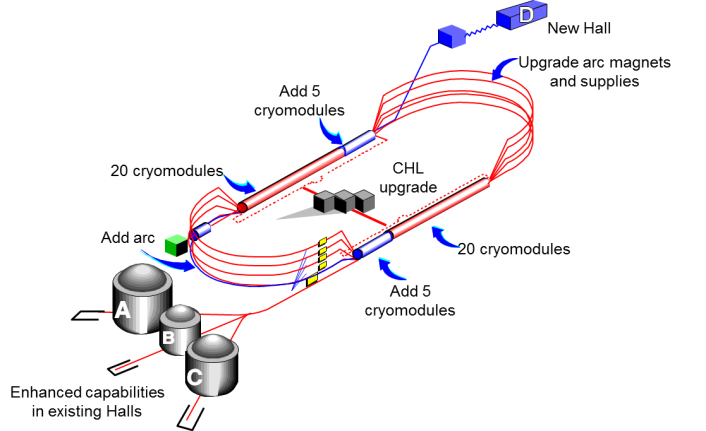
\includegraphics[width=0.8\linewidth]{figures/cebaf.png}
	\caption{CEBAF upgraded for the 12 GeV era.}
	\label{fig:cebaf}
\end{figure}

\section{Continuous Electron Beam Accelerator Facility}
The construction of the Continuous Electron Beam Accelerator Facility (CEBAF) completed in 1994. It originally consisted of two antiparallel linear accelerators (LINACs) connected by nine recirculation arcs that accelerated electrons to an energy of 6 GeV at a current of up to 300 \textmu A. In 2004, JLab began an energy upgrade that would allow CEBAF to supply electrons up to 12 GeV. The same framework used for the 6 GeV accelerator would be used for the 12 GeV era. That is, each pass around the accelerator would increase the energies, which was 1-1.2 GeV/pass during the 6 GeV era \cite{clasnote:CEBAF} and 2.2 GeV/pass after the 12 GeV upgrade. Originally, that meant 5 passes would produce 6 GeV electrons before they were fed into the three existing experimental halls ($i.e.$ Hall A, Hall B, and Hall C). In addition to the energy upgrade that increases the energy, a new experimental hall was built ($i.e.$ Hall D). That leads to 5 passes creating an 11 GeV electron beam to Halls A, B and C. Hall D received electrons from 5.5 passes around the accelerator creating the 12 GeV electron beam energy. As Fig. \ref{fig:cebaf} shows, the upgrade consisted of addition 5 additional cryomodules, an additional recirculation arc, increased capacity of the Central Helium Liquefier (CHL), and improvements in the curving magnet.

These electrons are accelerated in CEBAF by way of the LINACs. These LINACs contain a set of superconducting Niobium accelerating cavities with a magnetic field that oscillates at a frequency of 1.5 GHz. Electrons are injected in bunches into the accelerator with an energy of 45 MeV at the same frequency as the cavities every 0.7 ns. These electrons then circulate around, increasing in energy each pass by the LINACs. Once the desired energy for a given hall is reached, the electrons are then received by the hall every 2.1 ns To go a given hall, magnetic fields inside the arcs force the electrons into specific central trajectories that guides them into that hall. The beam is considered "continuous" because of the high operating frequency at which is can operate up to its maximum capacity at 200 \textmu A.
 
\section{CEBAF Large Acceptance Spectrometer}
Once the electrons are accelerated to a desired energy, they are received by the halls, where they enter each hall's spectrometer. A spectrometer is just an instrument (or collection of instruments) that measure and analyze a range (or spectrum) of processes or reactions. Because BONuS12 will operate in Hall B, here we will focus on the components and operation of Hall B's spectrometer, called the CEBAF Large Acceptance Spectrometer at 12 GeV (or CLAS12). As the name suggests, CLAS12 is an evolution of CLAS6 (or just CLAS as it was known before talk of the energy upgrade), which was the original spectrometer built for Hall B. 

\begin{figure}[h!]
	\centering
	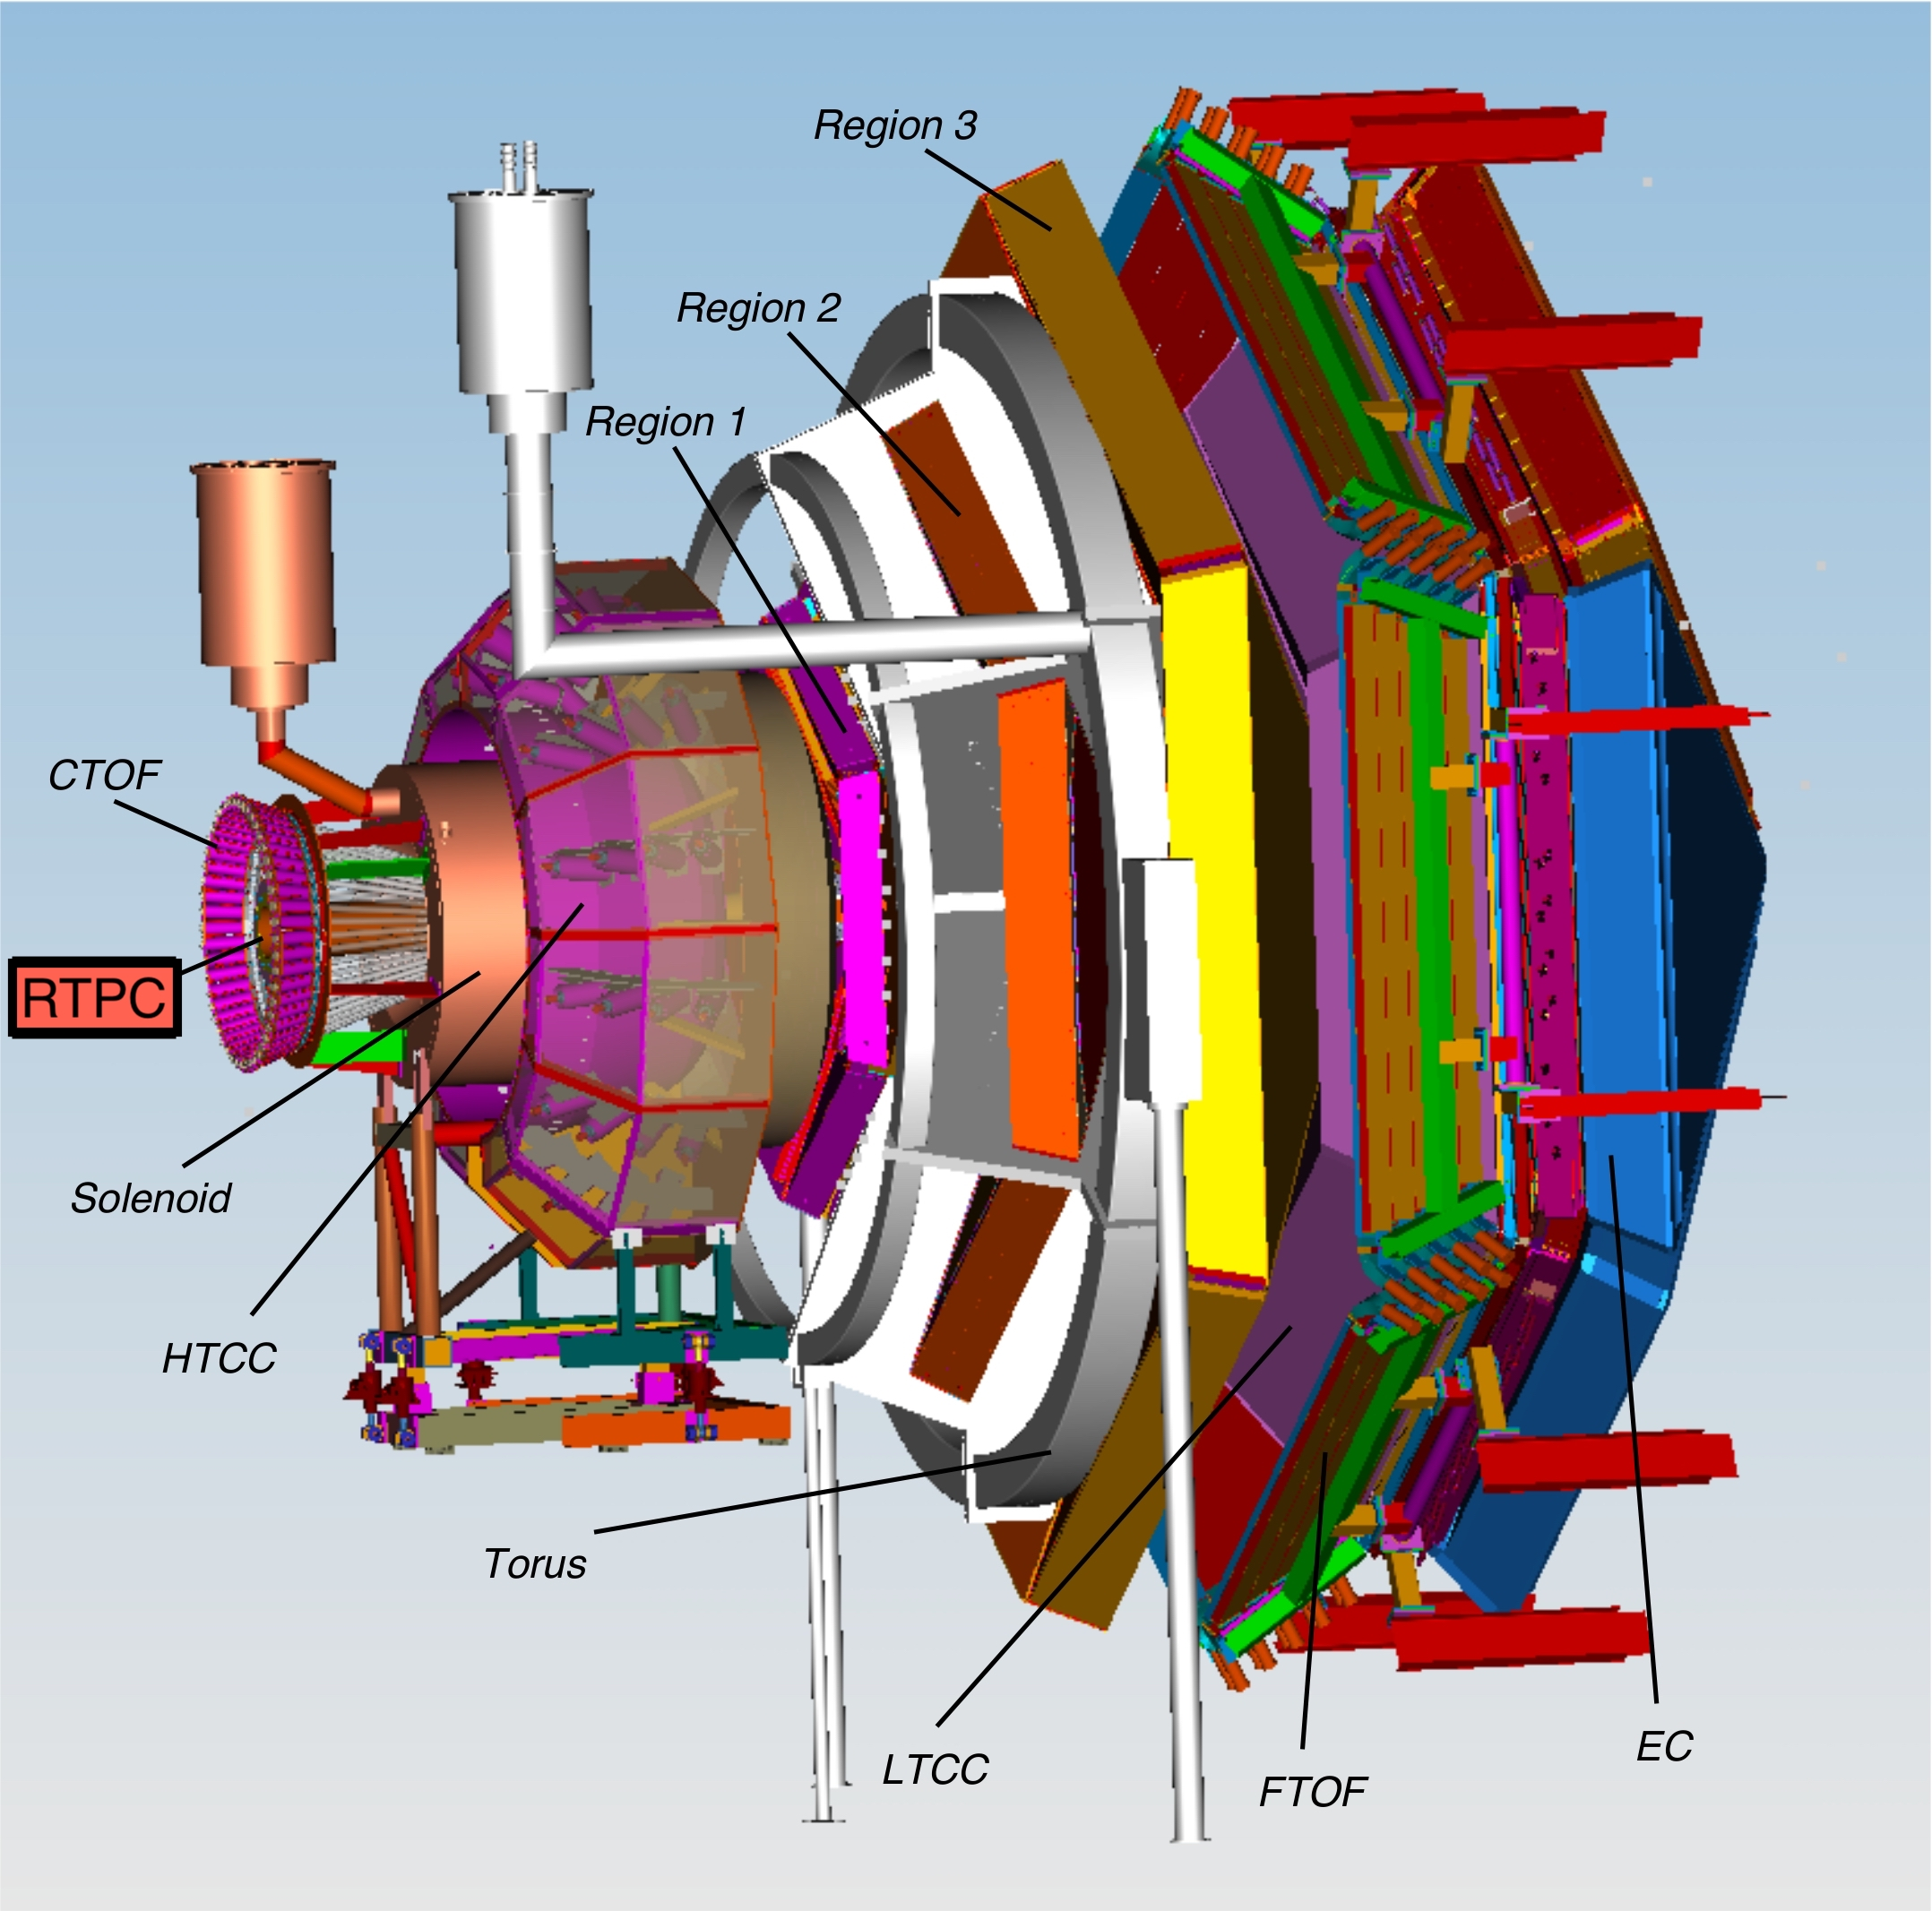
\includegraphics[width=0.8\linewidth]{figures/clas12.png}
	\caption{The CEBAF Large Acceptance Spectrometer at 12 GeV (CLAS12).}
	\label{fig:clas12}
\end{figure}

CLAS12 (see Fig. \ref{fig:clas12}) consists of two major groups of detectors, which together allow for detection and identification of particles over a large scattering angle, thus the "Large Acceptance" words in the name CLAS12. The Forward Detector (FD) covers scattering angles of between 5-40 degrees, and consists of a torus magnet, Cherenkov counters, a time of flight detector, drift chambers and electromagnetic calorimeter. The other group of detectors is known as the Central Detector (CD), which covers scattering angles between 40-125 degrees. The CD consists of a solenoid magnet, time of flight detector and finally, the BONuS12 RTPC. We will discuss each of these detectors, with a bit more focus on the RTPC.

\subsection{Torus Magnet}
The torus magnet is comprised of six superconducting coils arranged symmetrically around the beamline to create a azimuthally symmetric magnetic field up to 3.5 T. The coils are cooled to an operating temperature of 4.5 K by liquid helium. The shape of the coils was designed to create a field that increases near the center, which provides the desired resolution as a function of $\theta$.

The purpose of the magnetic field is to curve the tracks of charged particles without changing their azimuthal ($\phi$) angle. This curvature allows for the increased capability of particle identification. Its open structure allows for long path lengths for both charged and neutral particles, which also contributes to particle identification through time-of-flight measurements.

\subsection{Cherenkov Counters}
When a charged particle moves through a dialectric\footnote{A dialectric is any insulator that can be polarized when an electric field is applied.} with a speed greater than the phase velocity of light in that medium, electromagnetic radiation ($i.e.$ light) is emitted. This is known as Cherenkov radiation. By changing the refractive index of that medium, the threshold for emission of that light is modified. This effect allows for the distinction of particles having the same energy and momentum. By using a material with a specific refractive index, a heavier particle may not produce Cherenkov light, but a lighter particle may.

\begin{wrapfigure}{L}{0.35\linewidth}
	\centering
	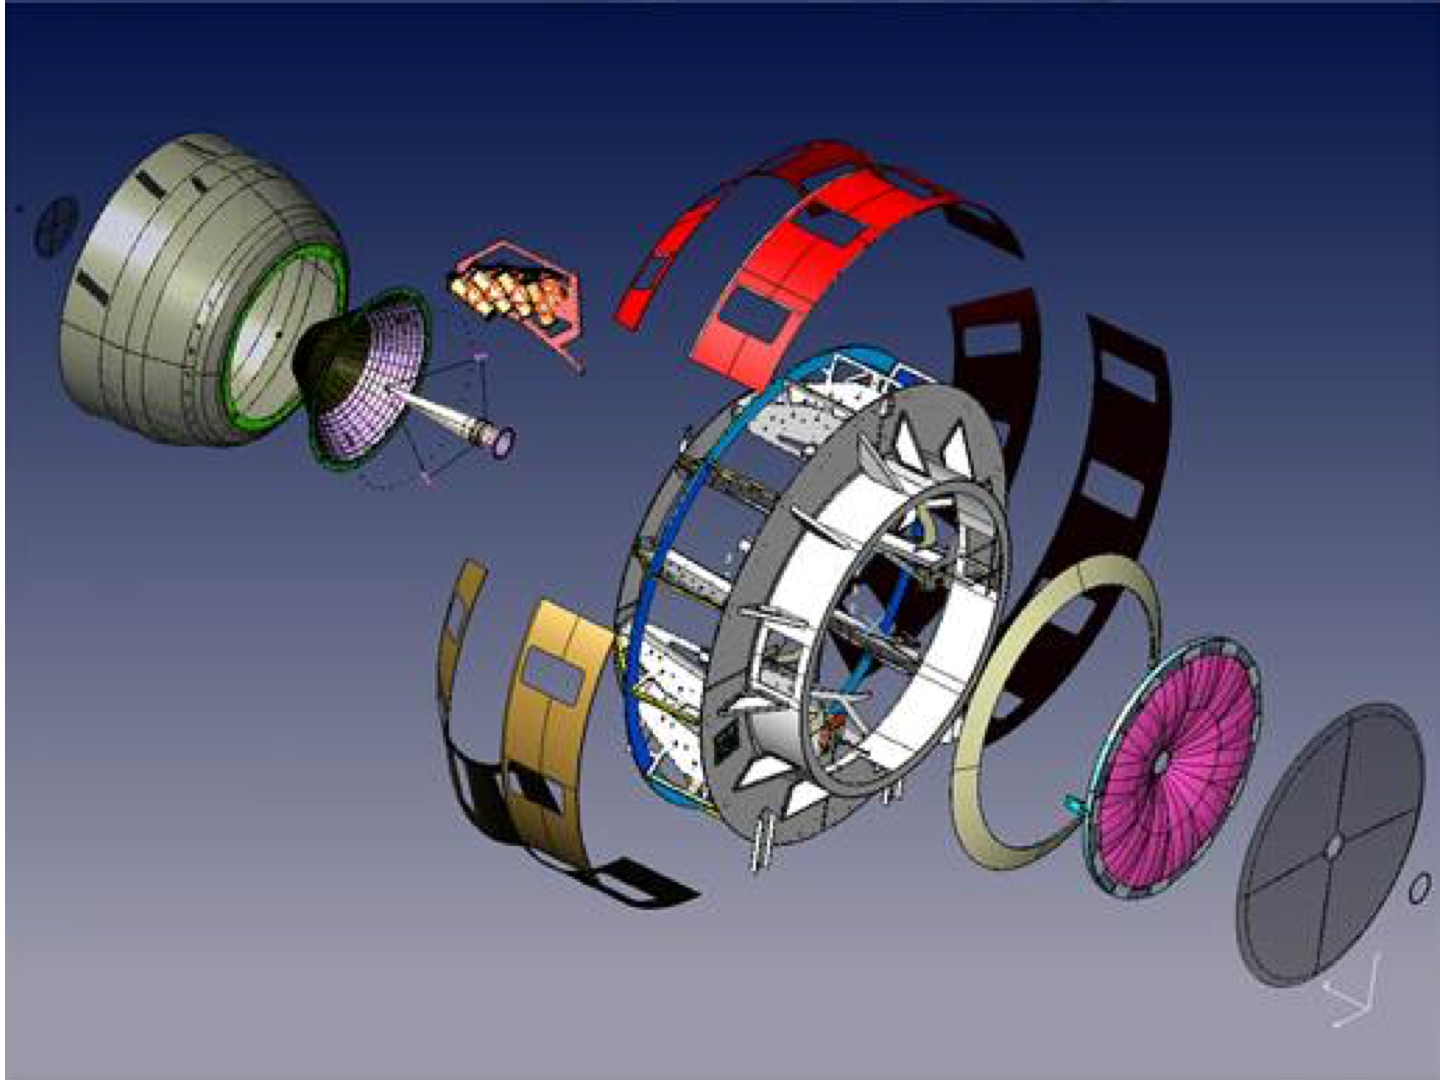
\includegraphics[width=0.9\linewidth]{figures/htcc.png}
	\caption{\label{fig:htcc}The High Threshold Cerenkov Counter.}
\end{wrapfigure}
CLAS12 contains two detectors that exploit this Cherenkov effect. The High Threshold Cherenkov Counter (HTCC seen exploded in Fig. \ref{fig:htcc}) is between the solenoid and the first region of the Drift Chambers. It discriminates electrons and pions by being filled with CO$_2$. This gas has an index of refraction $n=1.00041$, which forces pion above 4.6 GeV to produce light. If the particle has an energy below this threshold and it produces light, it is an electron. The other Cherenkov detector is the Low Threshold Cerenkov Counter (LTCC), which sits between Region 3 of the Drift Chambers and the Forward Time of Flight detector. It is filled with C$_4$F$_12$, which allows for the discrimination of pions and kaons at the 2.6 GeV where only pions produce Cherenkov light.

\subsection{Drift Chambers}
There are three regions of Drift Chambers (DC) that collectively allow for the reconstruction of charged particle trajectories. The first region is located in front of the Torus Magnet out the reach of the field. Region 2 is between the coils in the high field region. The third region is after the Torus, but feels a small magnetic field from the coils. Each region is made of six triangular sectors, which are made of small wires and filled with a gas mixture that exploits the process of ionization.

Within the sectors of the DC there are hundreds of wires, half of which are positive and the other half negative. When a charged particle travels through the gas mixture (90$\%$ Argon 10$\%$ CO$_2$ for the case of the CLAS12 DC), it knocks off electrons from the gas molecules as it passes. This process is known as $ionization$. In the DC, these ionization electrons that are created as charged particles pass through are accelerated to the nearest positive wire from the electric field created by the negative-positive wire pairs. The ion created is accelerated toward the nearest negative wire by the same electric field.

Using the signals created by the electron-ion pairs as the charged particle travels through the regions of the DC allow for the reconstruction of that particle's path. This information lends itself to the reconstruction of the particle momentum as well as its vertex ($i.e.$ where the particle collision occurred). This information will be vital in BONuS12 for identifying the electron created in the $eD \rightarrow e'p_sX$ process.

\subsection{Forward Time of Flight}
Two charged particles having the same momentum will travel at different speeds depending on their mass. The Forward Time of Flight detector (FTOF) will measure the time of arrival of those charged particles emerging from the target. Primarily, the FTOF will help separate between pions and kaons for energies below 3 GeV. Higher energies are handled by the Cherenkov counters. Because higher momentum particles scatter at lower angles, the FTOF was constructed to have better timing resolution at lower angles. That resolution can be as small as 80 ps at the more forward angles and 150 ps at larger angles ($i.e.$ over 35 degrees).

The FTOF is made of six sectors of plastic scintillators coupled to double-sides PMT readout. Within each sector, there are three arrays of counters. Panel 1a, which covers 5 to 35 degrees in $\theta$ contains 23 counters. Panel 1b also covers angles between 5 and 35 degrees and contains 62 counters. Finally, Panel 2 has 5 counters covering only angles between 35 and 45 degrees. 

\subsection{Electromagnetic Calorimeter}
Electromagnetic calorimeters measure the energy of particles traveling through it that interact via the electromagnetic interaction. The EC in CLAS12 contains three layers. The preshower calorimeter (PCAL) is the first layer and is used to identify two close gammas, which will help discriminate between neutral pions and single gammas. The next two layers are the inner and outer electromagnetic calorimeters (IC and OC, respectively). Both are used collectively with the PCAL to identify electrons, photons, $\pi^0 \rightarrow \gamma \gamma$, and neutrons.

\begin{figure}[h!]
	\centering
	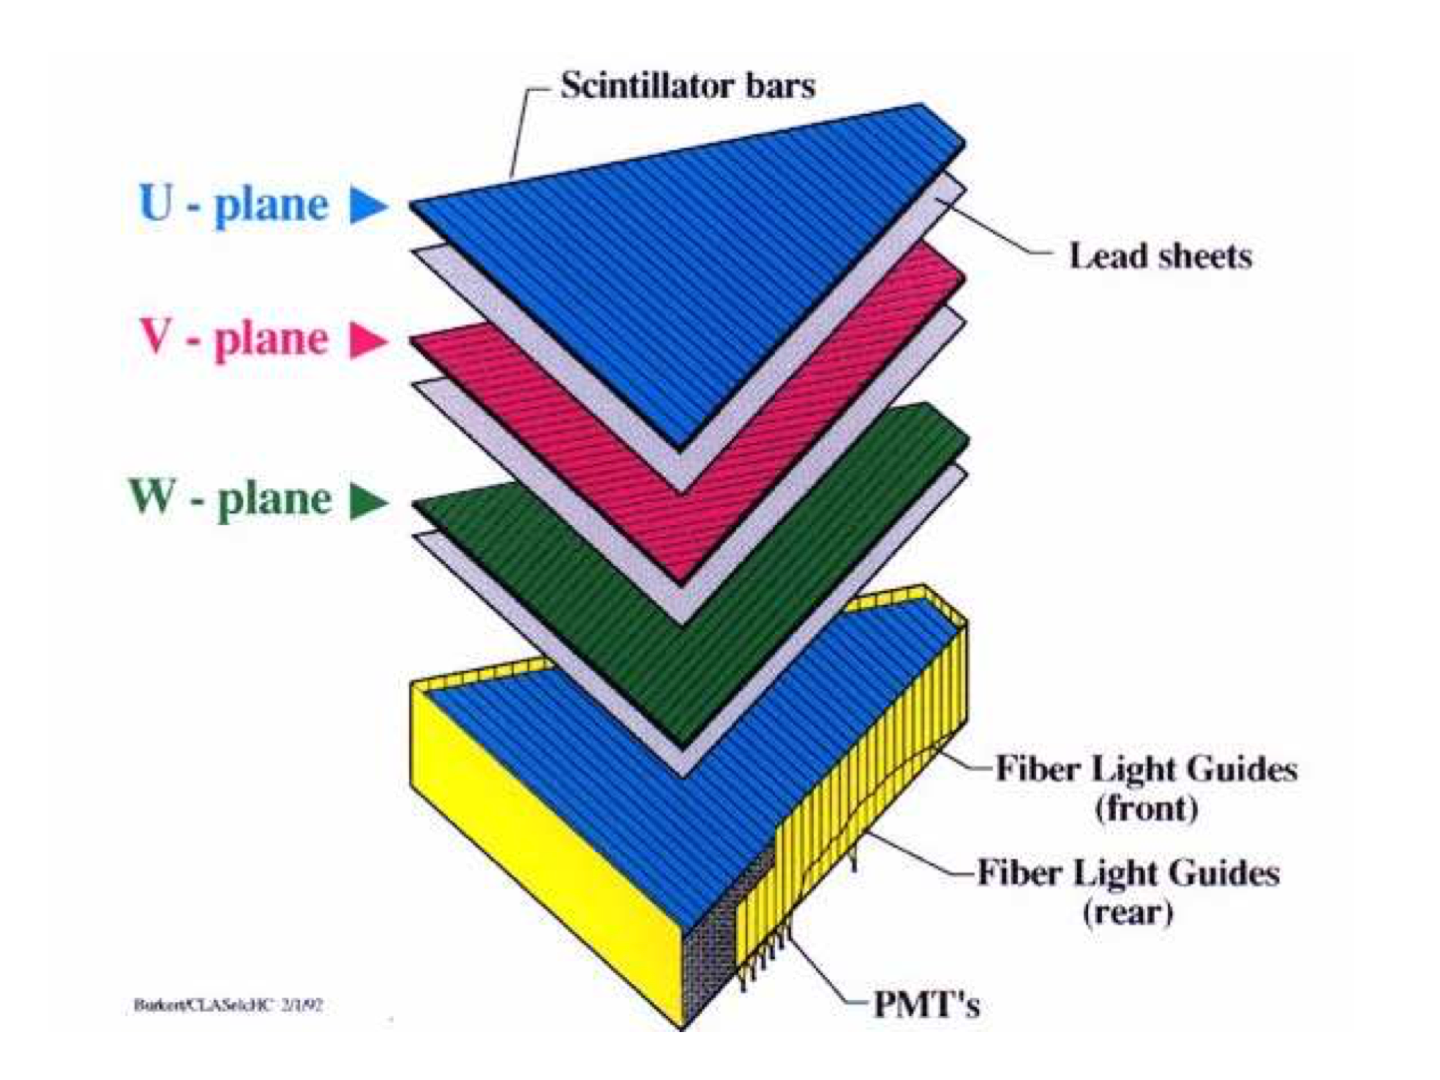
\includegraphics[width=0.8\linewidth]{figures/ecal.png}
	\caption{Exploded view of a sector of the Electromagnetic Calorimeter (EC) for CLAS12. \cite{clasnote:EC_geo} }
	\label{fig:ecal}
\end{figure}

The requirements of the EC are to identify the electrons with energies above 0.5 GeV, and measurements of photons above 0.2 GeV helping to reconstruct $\pi^0$ and $\eta$ particles through their neutral decays. The EC can also provide photon/neutron separation by utilizing TOF information available.

Each layer of the EC is comprised of six triangular sectors. Each sector is made of alternating layers of scintillators strips and lead sheets. The geometric readout comes from the three planes seen in the exploded view of one sector in Fig. \ref{fig:ecal}, that is U, V, and W planes. In each plane, there are 36 scintillator strips that run parallel to one side of the nearly equilateral triangular sectors. Strips are rotated by 120$^{\circ}$ in each successive layer, which allows for effective translation to x, y, and z coordinates.  

\subsection{Solenoid Magnet}
The solenoid magnet and the remaining two detectors to follow ($i.e.$ the Central Time of Flight and Radial Time Projection Chamber) are all members of the group known as the Central Detector. The Solenoid is a super-conducting magnet cylindrical in shape that surrounds the beam line. It is capable of producing a field of up to 5 T along the beam line. Charged particles experiencing this field curve in a helical trajectory, which allows for reconstruction of those trajectories and discriminates between charged and neutral particles.

The other purpose of the solenoid is to shield the Forward Detector from electron-electron collisions, called M\o ller electrons. Because the the field is strongest closest to the target, most M\o ller electrons originating from the beam line are isolated from the solenoid's field to small polar angles ($\theta$) where none of the FD materials begin. The other means of protection from these M\o llers come from a shield around the beam line located just after the Central Detector as well as a shield just in front of a small detector called the Forward Tracker, which for the BONuS12 Experiment will be turned off.
 
\subsection{Central Time of Flight}
\begin{wrapfigure}{R}{0.35\linewidth}
	\centering
	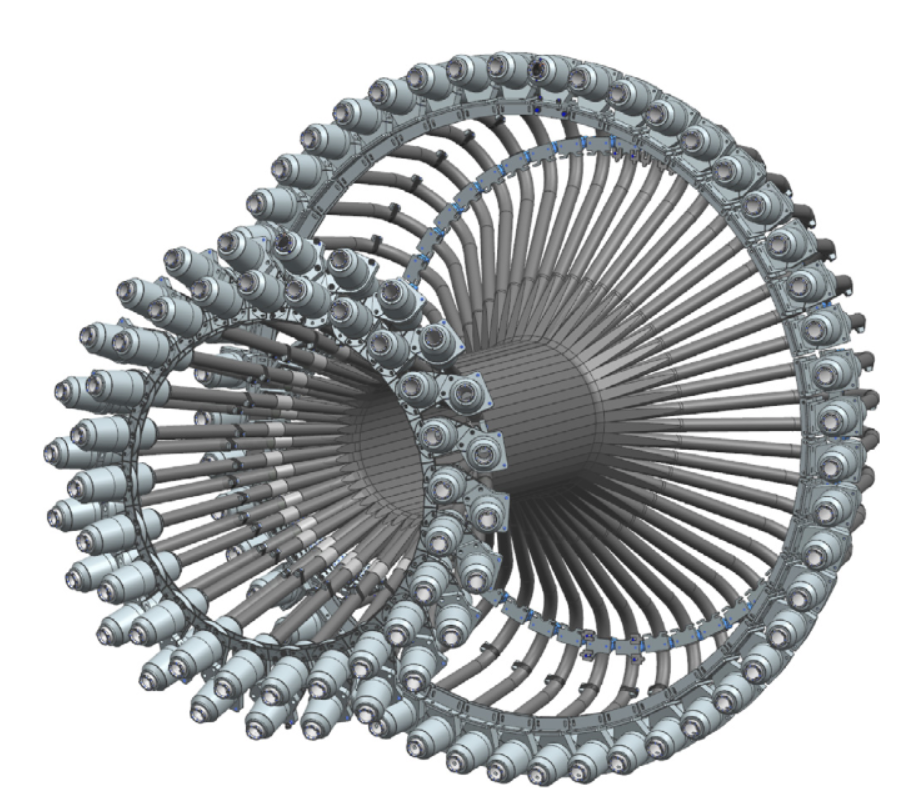
\includegraphics[width=0.9\linewidth]{figures/ctof.png}
	\caption{\label{fig:ctof}The Central Time of Flight Detector.}
\end{wrapfigure}

The Central Time of Flight (Fig. \ref{fig:ctof}), just as the FTOF, measures the time of flight of particles originating at the reaction vertex. It is made of 48 scintillator bars that form a barrel and spans polar angles of 35$^{\circ}$ to 125$^{\circ}$ that surround the target with full azimuthal coverage. The scintillators are coupled on each end by magnetic-field-sensitive PMTs, which are positioned out of the solenoids field by long light guides. The resulting CTOF operates with a time resolution of 60 ps, which was the requirement for particle identification.

\section{BONuS12 RTPC}
During Run Group F (RGF) in Hall B at JLab all of the detectors just described will be present in addition to one more that will be located inside the solenoid magnet whose outer limits end just before the CTOF. That detector is the BONuS12 Radial Time Projection Chamber (or RTPC). Its purpose is detect protons by way of ionization electrons created as protons pass through the RTPC.

\subsection{Components and their Purpose}
Accelerated electrons that enter Hall B hit the RGF designated target. That target measures 3 mm radially is made gaseous Deuterium target at 7 atm pressure surrounded by a 65 \textmu m thick Kapton wall. When an electron collides with a neutron in a deuteron atom, it continues in the forward direction into the Forward Detector of CLAS12. That collision also results in the ejection of a proton that drifts radially outward into the RTPC.

\begin{figure}[h!]
	\centering
	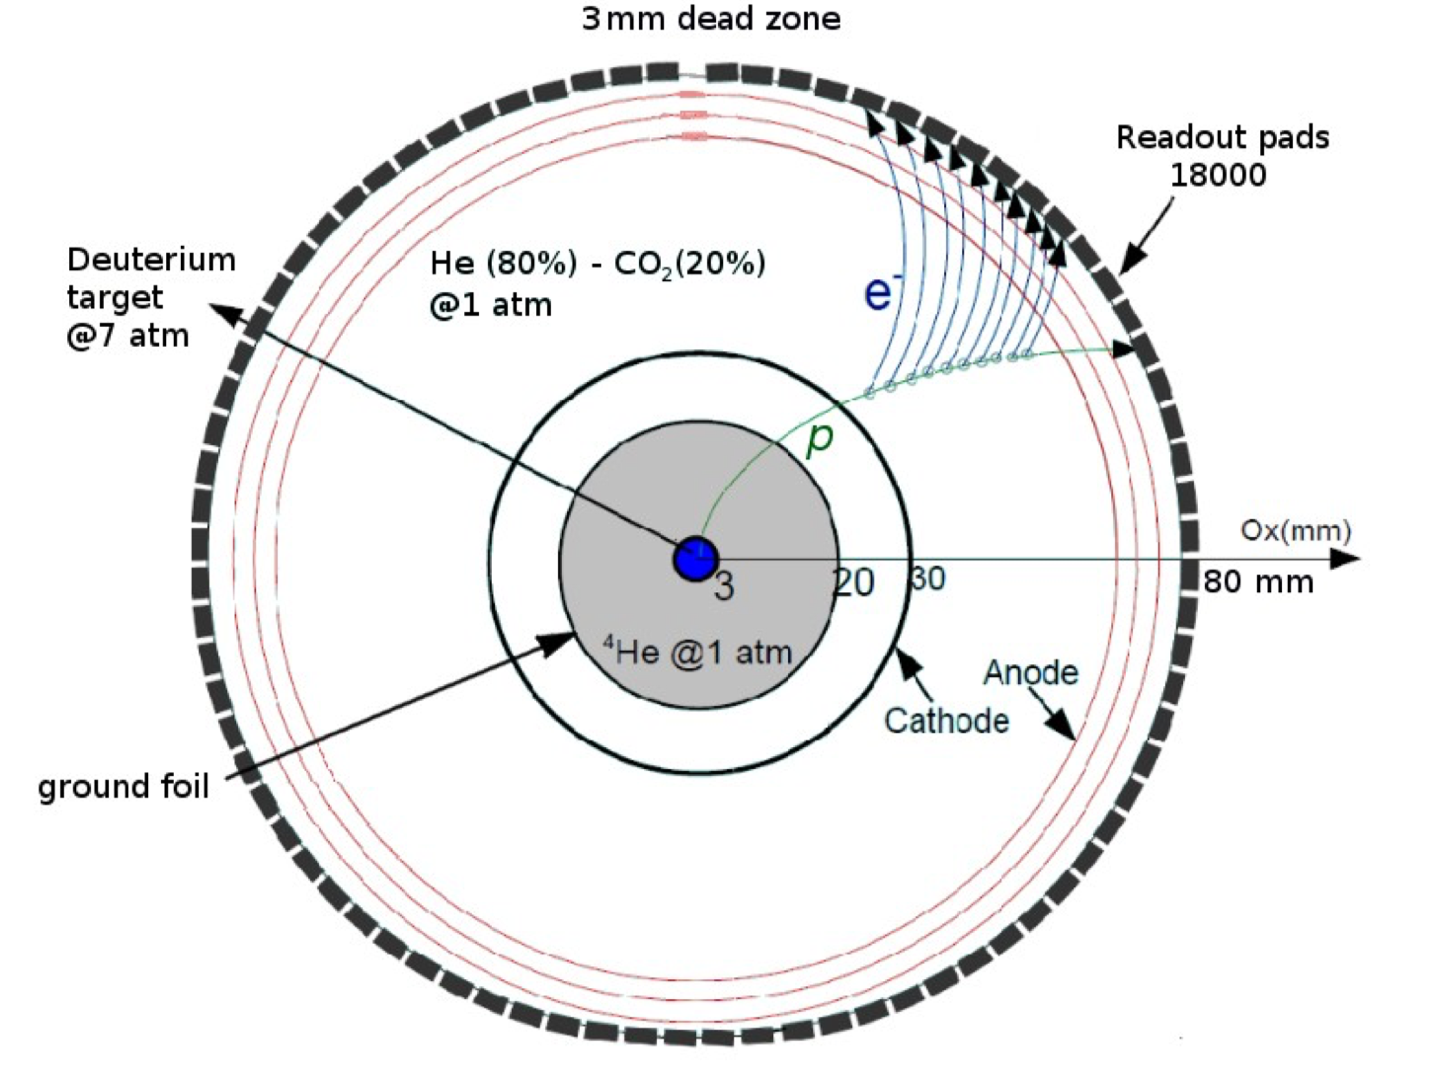
\includegraphics[width=0.8\linewidth]{figures/rtpc_op.png}
	\caption{Cross section of the RTPC showing a proton traversing the detector with ionization electrons drifting toward the readout pad board.}
	\label{fig:rtpc_op}
\end{figure}

That proton is guided toward the outer edge of the RTPC by way of an electric field created within the RTPC. That field is established with a ground foil at 2 cm and a cathode foil at 3 cm. The cathode foil is given a high negative potential and the ground foil is inherently at zero potential. This potential difference creates that electric field through the active region of the RTPC, which begins at the cathode foil and ends at the first Gaseous Electron Multiplier (GEM) foil. 

This active region is where the proton will create ionizations along its path outward. This region is filled with a gas mixture of 80$\%$ Helium and 20$\%$ CO$_2$, which was chosen for its fast drift times and minimal drift angle (more about this in Section \ref{sec:gas_opt}). Because of the magnetic field created by the solenoid, the proton curves in one direction as it moves outward while the ionization electrons it creates curve in the opposite direction due to their opposite charge.

Every time an ionization electron is created, it is also driven by the electric field toward the outer edge of the RTPC where readout pad board waits for its arrival. However, because a single electron cannot be easily readout, that electron will encounter three layers of GEM foils at 7 cm, 7.3 cm and 7.6 cm. Those GEMs are used to amplify the number electrons from one to something significant enough to register on the electronics. Each GEM has a gain of about 100, which means that through three GEM layers, one electron could become 10,000 after exiting the last layer.

\begin{figure}[h!]
	\centering
	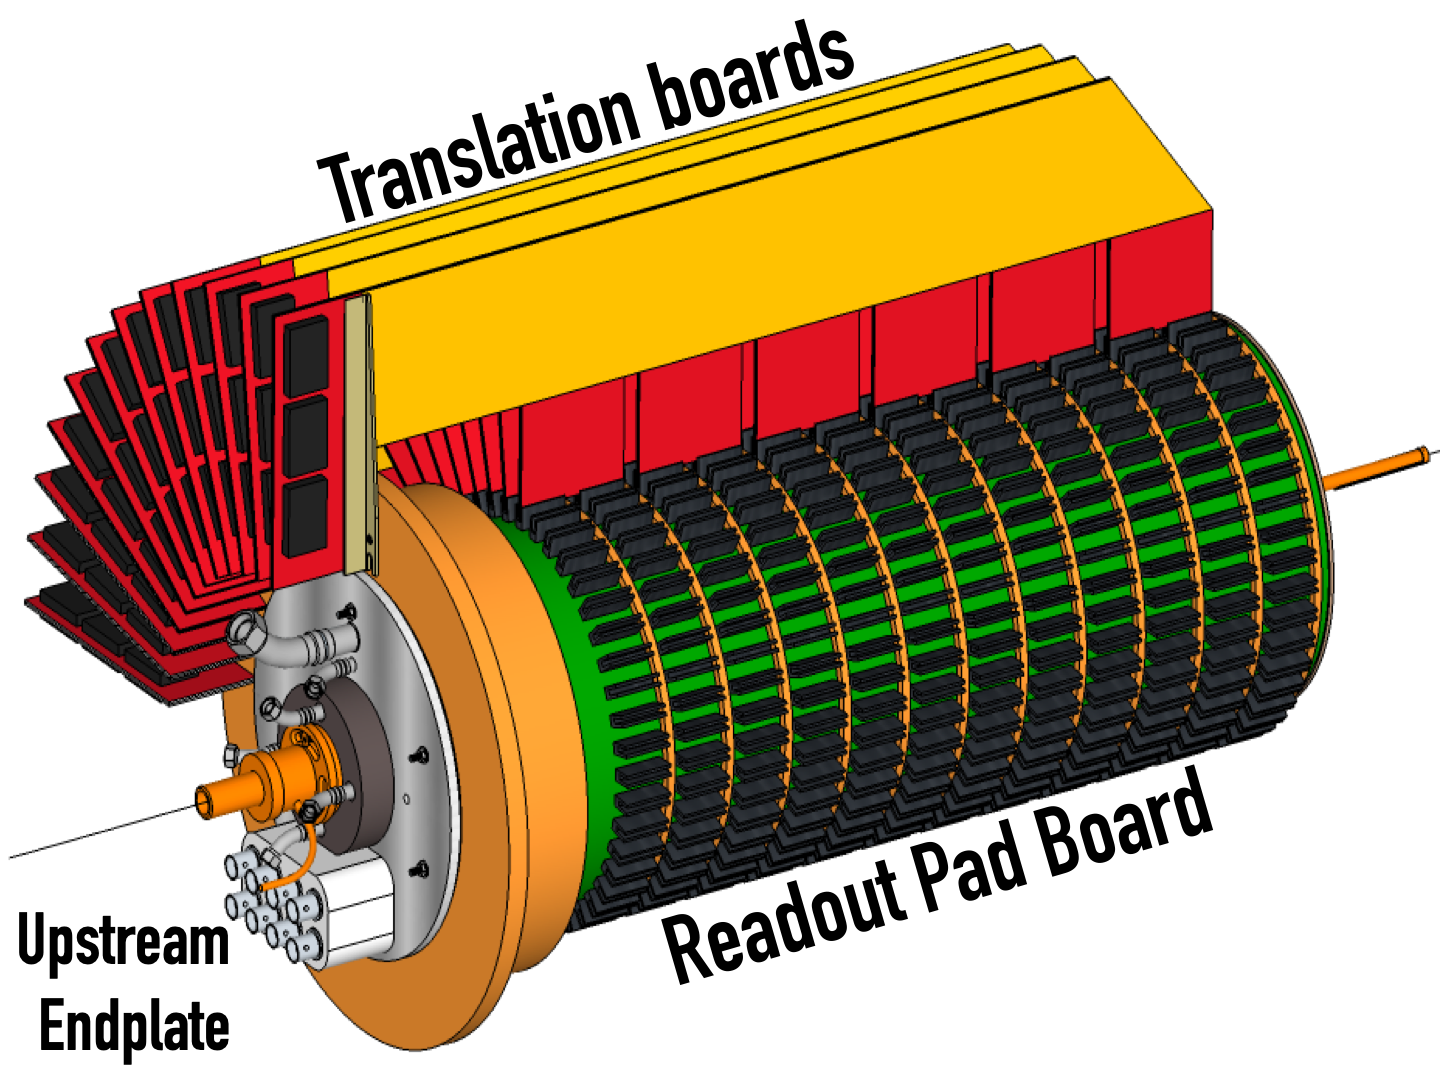
\includegraphics[width=0.8\linewidth]{figures/rtpc_design.png}
	\caption{Design of the RTPC with only one-quarter of the translation boards attached.}
	\label{fig:rtpc_design}
\end{figure}

Once this avalanche of electrons has been created by the GEMs, their final destination is the read out pad board at 8 cm. The pad board has 180 pads around $\phi$ by 96 pads in $z$ totaling 17,280 readout pads. These pads, coupled to translation boards that act as current-limiting adapter boards the electronics, reads the signal that the electron avalanche makes. The electronics It then gets driven to the data acquisition system, which stores the data for analysis.

\subsection{BONuS12 RTPC Drift-gas Monitoring System}
The drift velocity of electrons in the RTPC is very sensitive to fluctuations in the gas-mixture and potential, as well as the temperature and pressure of the gas in the active region (see \ref{sec:gas_opt}). Therefore, a system was designed that monitors the drift velocity of electrons in the gas mixture of the active region in the RTPC. To achieve this, a small drift chamber was designed whose gas mixture would come from downstream of the RTPC.

\begin{figure}[h!]
	\centering
	\includegraphics[width=0.8\linewidth]{figures/dms_concept.png}
	\caption{Design concept of the Drift-gas Monitoring System (DMS) for the BONuS12 Experiment.}
	\label{fig:dms_concept}
\end{figure}

Since the purpose of this Drift-gas Monitoring System (DMS) is to measure the drift velocity within the gas mixture, the focus of the DMS design was measuring that velocity through a near-constant electric field. The design concept (seen in Fig. \ref{fig:dms_concept}) is a drift chamber where two sources at a known distance between them emits $\beta$ electrons up to associated scintillator/PMTs. When these electrons travel through the gas, they create ionization electrons along their path. Within a sensitive region in the center of the DMS, those ionization electrons are guided to an anode wire behind a small slit in a grounded plate by an electric field. 

The electric field that guides the ionization electrons to the anode is created by a cathode with a high negative potential, an anode with a high positive potential, and field-shaping electrodes that have potentials stepped down by equal amounts from a voltage-divider circuit. This ensures the field within that sensitive region is uniform, so no unwanted acceleration of electrons occurs between the two sources.

\begin{figure}[h!]
	\centering
	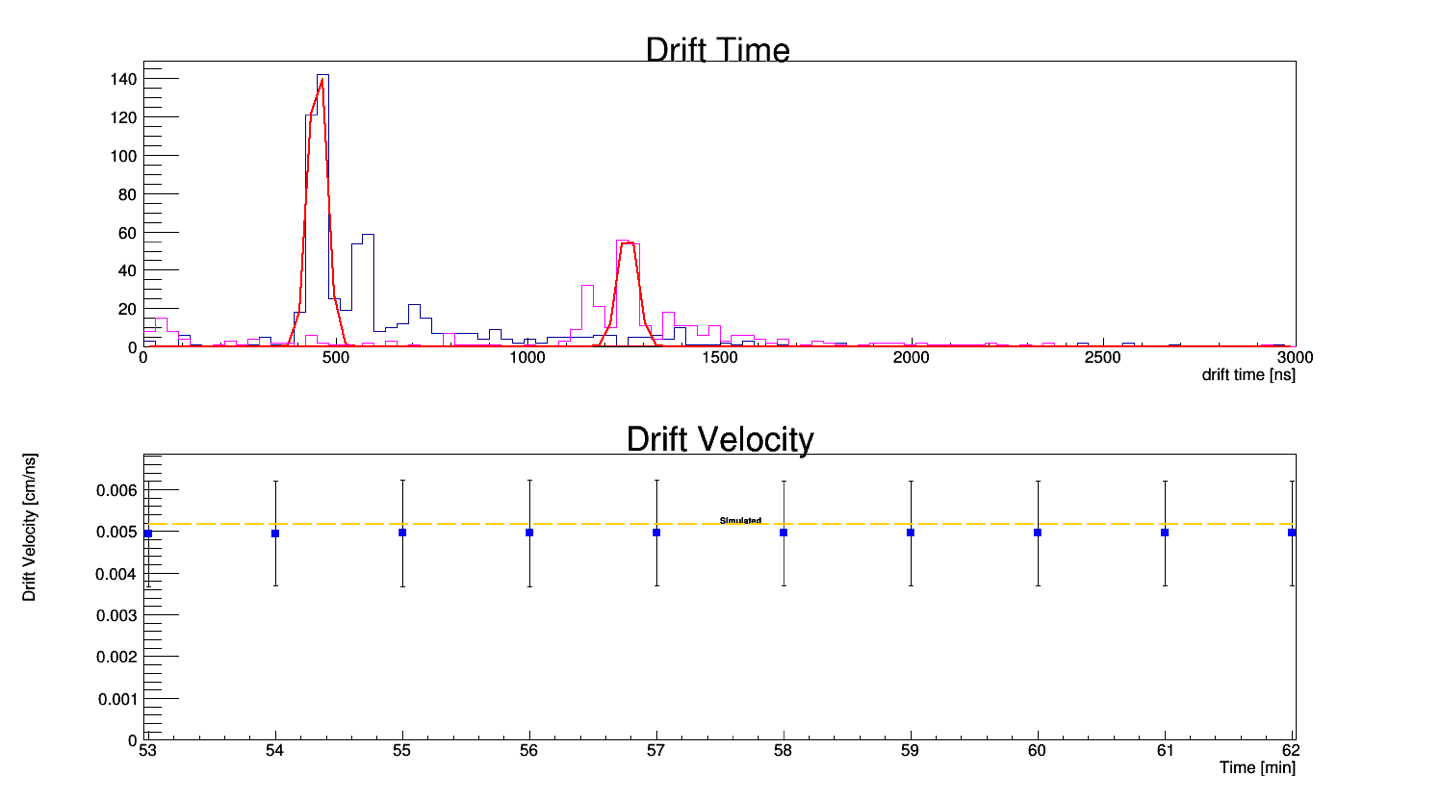
\includegraphics[width=0.8\linewidth]{figures/dms_gui.png}
	\caption{Monitoring output of the DMS.}
	\label{fig:dms_gui}
\end{figure}

When a source $\beta$ electron is detected by either PMT, a Time-to-Digital Converter (TDC) looks for an associated ionization electron at the anode. When a signal on the anode is seen, the TDC adds that drift time to a histogram. As enough statistic populate the histogram, two peaks are formed from the drift of electrons from the two sources and then a difference in the two times can be calculated. Given the known distance between the sources and the time difference between the two peaks, the drift velocity is calculated. Then the drift velocity is plotted versus time elapsed, giving a means to monitor that velocity (see Fig. \ref{fig:dms_gui} for those plots from DMS testing).

\subsection{Construction and Integration}
The construction of the BONuS12 RTPC was completed at Hampton University in Hampton, Virginia around 2017. Because of the cylindrical shape of the detector, mandrels were used widely in the shaping of the detector components. The ground foil, cathode foil, the three layers of GEM foils, and pad board were all assembled using mandrels. Fig. \ref{fig:rtpc_assembly} is a drawing of the assembly station for the RTPC, which includes an actuator that removes wrapped foils from the mandrel and places the into the detector on the assembly station.

\begin{figure}[h!]
	\centering
	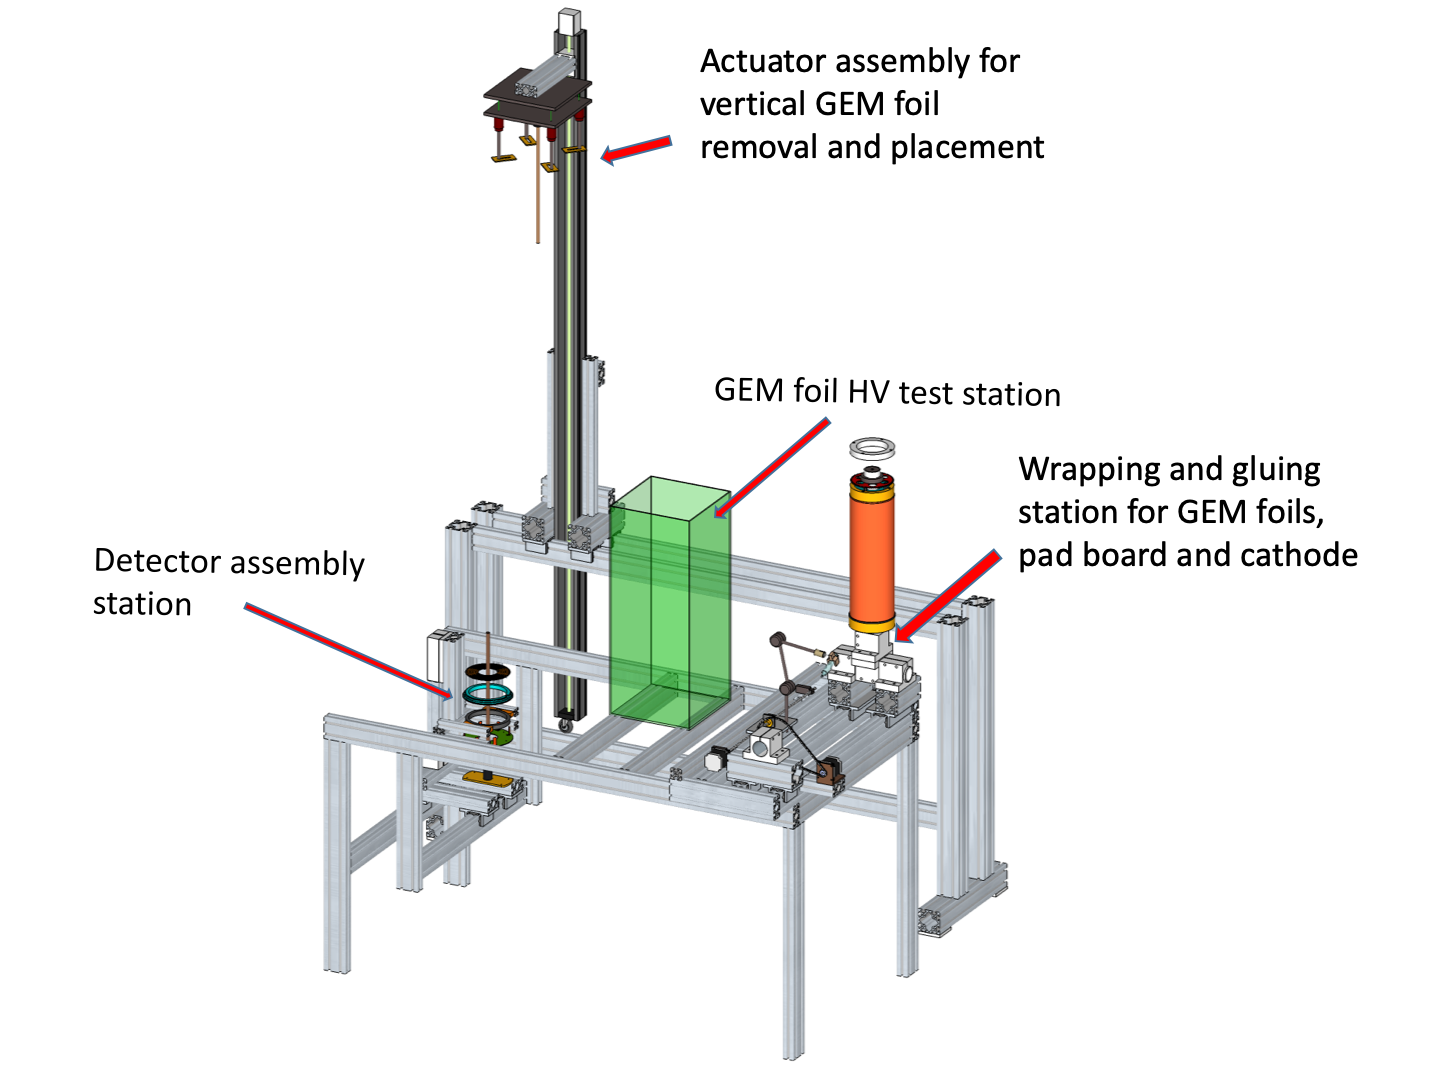
\includegraphics[width=0.8\linewidth]{figures/rtpc_assembly.png}
	\caption{Assembly station for the RTPC.}
	\label{fig:rtpc_assembly}
\end{figure}

The first assembled detector was delivered to JLab in November 2019. The Drift-gas Monitoring was also delivered to JLab in November 2019. Both are undergoing testing in the Experimental Equipment Lab (EEL) with the full array of components that will be installed in the Experimental Hall ($i.e.$ RTPC, gas panel including the DMS, DAQ, etc). Once that testing is complete, in late January 2020 the BONuS12 RTPC will be installed in Hall B. Run Group F, of which the BONuS12 Experiment is a part, will also require the installation of three layers of the Forward Micromegas Tracker, switching the Forward Tagger to the FTOff M\o ller Shield, as well as cabling for all of those installed detectors. Once this is complete, cosmic ray testing will begin. This will allow for the first data stream of the RTPC from within the CLAS12 Data Acquisition System whilst inside the hall. Then on 12 February 2020, Run Group F will begin and BONuS12 will begin taking data. 